\begin{figure}[!ht]
    \centering
    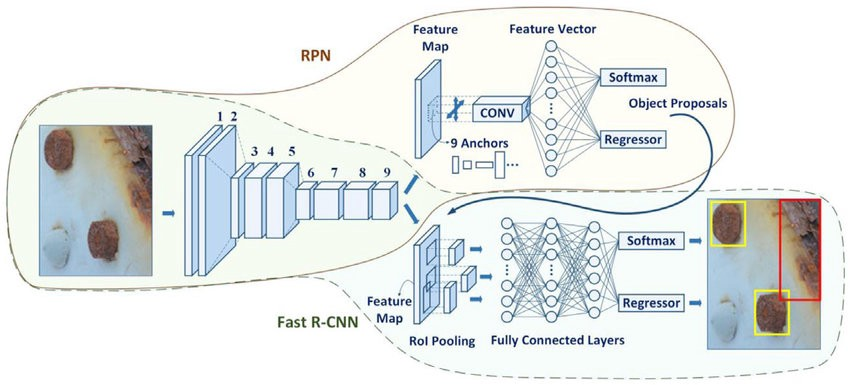
\includegraphics[width=0.9\textwidth]{chapter2/images/faster_rcnn.png}
    \caption[โครงสร้างทั่วไปของโมเดลปัญญาประดิษฐ์ของ Faster RCNN]{โครงสร้างทั่วไปของโมเดลปัญญาประดิษฐ์ของ Faster RCNN\textsuperscript{\cite{faster_pic}}}
    \label{fig:faster_rcnn_architecture}
\end{figure}
\par Faster-RCNN\textsuperscript{\cite{faster}} มีการพัฒนาในการหาพื้นที่ที่สนใจ (region of interest หรือ ROI) โดยเปลี่ยนจากใช้โครงข่ายหาพื้นที่ที่สนใจแยกเฉพาะ (selective search) นำมารวมในโครงข่ายเดียวกัน 
ดังนั้น Faster-RCNN จึงมีโครงข่ายประสาทเทียม (neural network) เดียวในการทำงาน ซึ่งภายในโครงข่ายจะประกอบไปด้วยการทำงานหลักสามอย่าง คือ
\begin{enumerate}
	\setlength\itemsep{-0.25em}
	\item การสกัดคุณลักษณะ
	\\	นำภาพเข้าชั้นคอนโวลูชันเพื่อการสกัดคุณลักษณะของภาพ
	\item การหาพื้นที่ที่คาดว่าจะมีวัตถุอยู่
	\\	หลังจากที่ภาพผ่านการสกัดคุณลักษณะแล้ว จะถูกนำเข้าไปใน region proposal network เพื่อหาพื้นที่ที่คาดว่าจะมีวัตถุอยู่
	\item การทำนายผล
	\\	ทำการ pooling คุณลักษณะของภาพและพื้นที่ที่คาดว่าจะมีวัตถุอยู่ และนำเข้าไปในชั้น fully connected จะได้ผลลัพธ์เป็นหมวดหมู่ของวัตถุและตำแหน่งของกรอบสี่เหลี่ยม  
\end{enumerate}
\par Region proposal network (RPN)\textsuperscript{\cite{faster}} คือ โครงข่ายที่หาพื้นที่ที่คาดว่าจะมีวัตถุอยู่จะถูกใช้หลังภาพผ่านการสกัดคุณลักษณะ ซึ่ง RPN มีโครงสร้างที่มีองค์ประกอบ 2 อย่าง
คือมีการบอกว่าบริเวณนั้นมีวัตถุอยู่หรือไม่ และสำหรับการระบุพิกัดของกรอบสี่เหลี่ยมที่คาดว่าจะมีวัตถุอยู่ ซึ่งผลลัพธ์จะได้เป็น ROI ของวัตถุในภาพ 